%% Models
%%=========================================

\chapter{Models}
\label{ch:models}
In this chapter we present the three models we created during our iterative development process. The models, ca

%%=========================================

\section{VectorRepeat}
The first model, called {\tt VecRep} for short, consists of two groups of LSTMs. The first group of LSTMs encodes the entire input and outputs its final hidden state. This hidden state is then repeated in the dimension of time, and inputted into a new group of LSTMs. 

With this approach, we can defin

The benefit of this approach is that we can define the width of the second LSTM to the width of our output. This is not possible when projecting the LSTMs hidden states, as described in the previous section, as the LSTM will have the same width for input and output.

\begin{figure}[ht]
    \centering
    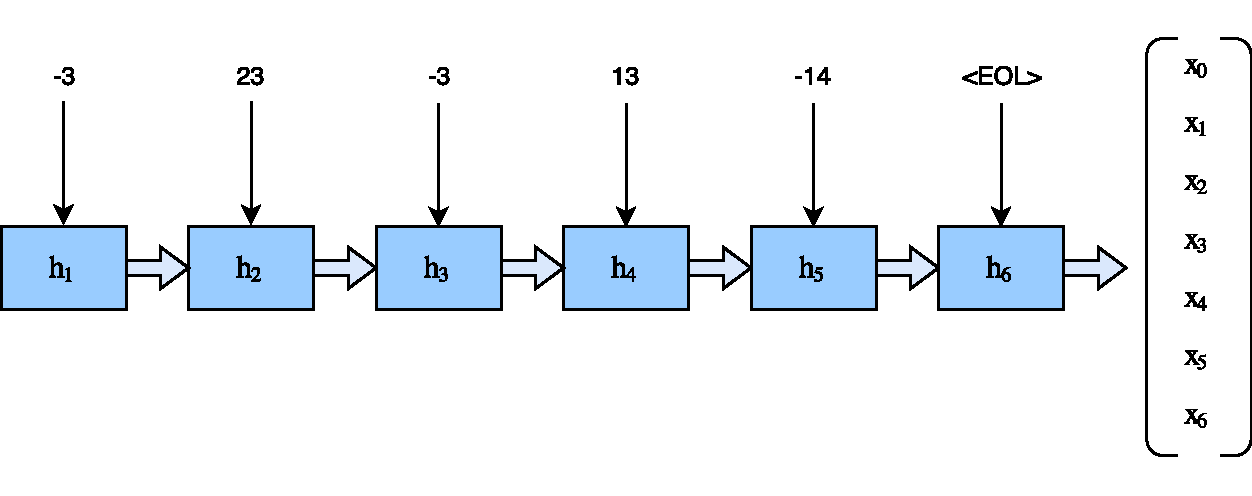
\includegraphics[width=0.7\textwidth]{fig/development_process/lstm-vector-projection-encoder.pdf}
    \caption{A LSTM outputting its final hidden state after reading a sequence}
    \label{fig:lstm-vector-projection-encoder}
\end{figure}

Figure \ref{fig:lstm-vector-projection-encoder} illustrates a regular LSTM that reads an input sequence and output its final hidden state. The output vector has a length equal to the width of the LSTM. As illustrated in Figure \ref{fig:lstm-vector-projection-decoder}, the hidden state from the LSTM is repeated \(n\) times, where \(n\) is the length of the output sequence. In this example, out output has a length of three characters, plus a special ``end of line" character. The resulting matrix of the repeated vector is then fed to another LSTM that reads each time step and output its hidden state for each iteration.

\begin{figure}[ht]
    \centering
    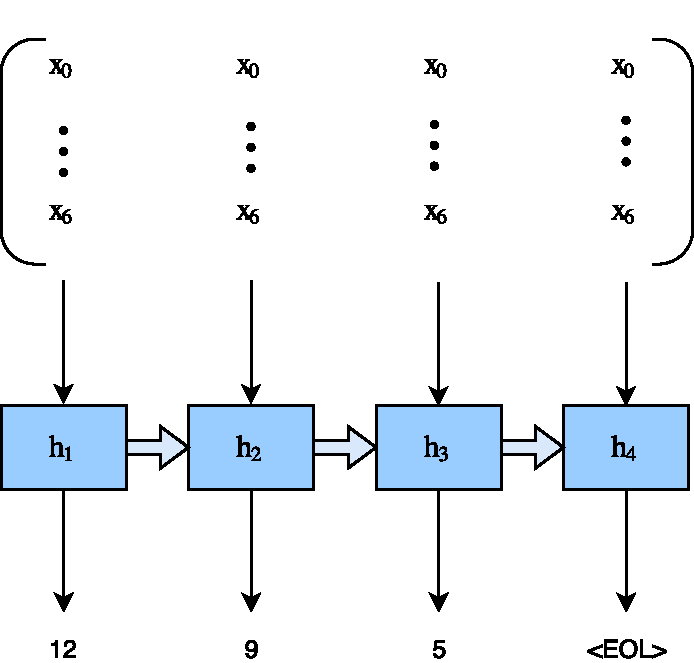
\includegraphics[width=0.5\textwidth]{fig/development_process/lstm-vector-projection-decoder.pdf}
    \caption{Repeating the output from a LSTM and feeding it to another LSTM}
    \label{fig:lstm-vector-projection-decoder}
\end{figure}

The vector approach is different from the one described in the previous iteration, and does not suffer from the same problem with alignment. Because we read the entire input sequence before anything is outputted, we no longer output anything that is dependent on data in future time steps. The vector from the first LSTM has essentially encoded the temporal dependencies in a single representation vector. This is not that different from how encoder-decoders create their fixed width context vector. The main difference between this approach and general encoder-decoders is that the output in the last LSTM is not fed back as input. This may cause problems because the output is not only dependent on the encoded input sequence, but also what it has already outputted.

%%=========================================

\section{EncDecReg}
\red{TODO}

%%=========================================

\section{EncDecAtt}
\red{TODO}